\section{Primal movement and the cost of a feasible dual solution}
\label{sec:primal-dual}

A short primal route to an accurate point need not extend to a short
route ending at a feasible primal--dual pair. We restate the
classical primal--dual geometry with its metric and endpoints explicit,
then compare the two on the dyadic linear program of
\cref{sec:discrete}.

\subsection{Speed allocation and the set of small-gap pairs}
Let $K$ be a proper cone (closed, pointed, full dimensional), and let $F$
be a standard self-concordant barrier satisfying
$F(tx)=F(x)-\nu\log t$ for $t>0$. Use the negative-pairing conjugate
\[
 F_*(s)=\sup_{x\in\interior K}\{-\ip{s}{x}-F(x)\},
 \qquad \widehat F(x,s)=F(x)+F_*(s).
\]
Consider the strictly feasible primal--dual pair
\[
 \min\{\ip{c}{x}:Ax=b,\ x\in K\},\qquad
 \max\{\ip{b}{y}:A^*y+s=c,\ s\in K^*\},
\]
and its exact centers $z(\eta)=(x(\eta),s(\eta))$, where
$s=-\eta^{-1}F'(x)$ and $\ip{x}{s}=\nu/\eta$.
Full primal--dual distances use the Hessian metric of $\widehat F$ on
the product cone, ignoring the affine constraints; distances
inside the feasible set can only be larger. A dot denotes
differentiation with respect to $\log\eta$.

\begin{proposition}[Classical speed allocation]
\label{prop:pd-split}
Put $H=F''(x)$, $g=H^{-1/2}F'(x)$, and let $\Pi_x$ be the Euclidean
orthogonal projector onto $H^{1/2}\ker A$. Then
\begin{align}
 \nu_{\rm P}(\eta)&:=\norm{\dot x}_{F,x}^2=\norm{\Pi_xg}^2,
 &\nu_{\rm D}(\eta)&:=\norm{\dot s}_{F_*,s}^2
       =\norm{(I-\Pi_x)g}^2,\notag\\
 \nu_{\rm P}(\eta)+\nu_{\rm D}(\eta)&=\nu.
 \label{eq:pd-split}
\end{align}
If $A$ has full row rank, then
\begin{equation}
 \nu_{\rm P}(\eta)=\eta^2\ip{c}{Mc},\qquad
 M=H^{-1}-H^{-1}A^*(AH^{-1}A^*)^{-1}AH^{-1}.
 \label{eq:activity-schur}
\end{equation}
Writing $p(\eta)=\ip{c}{x(\eta)}$ and
$d(\eta)=\ip{b}{y(\eta)}$, one has
\begin{equation}
 -\eta^2p'(\eta)=\nu_{\rm P}(\eta),\qquad
 \eta^2d'(\eta)=\nu_{\rm D}(\eta).
 \label{eq:objective-progress}
\end{equation}
If both objectives converge to the finite optimum $p^*$, then
\begin{equation}
 p(\eta)-p^*=\int_\eta^\infty\frac{\nu_{\rm P}(u)}{u^2}\dd u,
 \qquad
 p^*-d(\eta)=\int_\eta^\infty\frac{\nu_{\rm D}(u)}{u^2}\dd u.
 \label{eq:integrated-gap-allocation}
\end{equation}
\end{proposition}
\begin{proof}
Logarithmic homogeneity and conjugacy give
$Hx=-F'(x)$, $\norm{g}^2=\nu$, and
$F_*''(s)=\eta^2H^{-1}$. Differentiating the central relation yields
$\eta\dot s=F'(x)-H\dot x$.
Thus $v=H^{1/2}\dot x$ and
$d_0=\eta H^{-1/2}\dot s$ satisfy $g=v+d_0$.
Feasibility gives $v\in H^{1/2}\ker A$ and
$d_0\in(H^{1/2}\ker A)^\perp$, proving \eqref{eq:pd-split}.
Removing redundant equalities leaves the feasible tangent spaces unchanged.
With full row rank, differentiated primal stationarity gives $\dot x=-\eta Mc$;
$MHM=M$ proves \eqref{eq:activity-schur} and the first identity in
\eqref{eq:objective-progress}.
Differentiate $p-d=\nu/\eta$ to obtain the second, and integrate for
\eqref{eq:integrated-gap-allocation}.
\end{proof}
The constant total speed is the calculation behind the primal--dual
theorem of Nesterov and Todd~\cite[Theorems~4.1 and~5.2]{NesterovTodd2002}.
Metric projections and Hessian isometries between conjugate barriers
also appear in Ohara, Ishi, and
Tsuchiya~\cite[Sections~4--5]{OharaIshiTsuchiya2024}. These
formulas are not new; we use them to determine exactly how much of the
total speed belongs to the primal path.

\begin{theorem}[Classical distance to feasible small-gap points]
\label{thm:pd-gap-set}
Let $z_0=z(\eta_0)$ be an exact central point, with gap
$\Delta_0=\nu/\eta_0$. For $0<\eps<\Delta_0$, let $\mathcal Z_\eps$ be
the set of all strictly feasible primal--dual pairs with gap at most
$\eps$. Then
\begin{equation}
 \sqrt{\nu/2}\log\frac{\Delta_0}{\eps}
 \leq d_{\widehat F}(z_0,\mathcal Z_\eps)
 \leq \sqrt\nu\log\frac{\Delta_0}{\eps}.
 \label{eq:pd-gap-set}
\end{equation}
The upper bound is the length of the central path from $z_0$ to
$z(\nu/\eps)$. Hence, for $0<R<1$, every forward-$R$ sequence
from $z_0$ to $\mathcal Z_\eps$ has at least
\begin{equation}
 \frac{\sqrt{\nu/2}\log(\Delta_0/\eps)}{-\log(1-R)}
 \label{eq:pd-gap-count}
\end{equation}
steps, even if intermediate points violate the affine equations.
\end{theorem}
\begin{proof}
At a center $z_c=z(\eta)$, conjugacy gives
$F_*'(s_c)=-\eta x_c$ and
$\widehat F(z_c)=\nu\log\eta-\nu$.
For any feasible $z=(x,s)$, orthogonality of primal and dual feasible
differences gives $\ip{x-x_c}{s-s_c}=0$. Hence
\[
 D\widehat F(z_c)[z-z_c]
 =-\eta\{\ip{s_c}{x-x_c}+\ip{x_c}{s-s_c}\}
 =-\eta\{\gap(z)-\nu/\eta\}.
\]
At $\eta=\nu/\eps$, convexity proves that $z_c$ minimizes
$\widehat F$ on $\mathcal Z_\eps$.
In the product-cone metric, the dual norm of $D\widehat F$ is exactly
$\sqrt{2\nu}$, since each logarithmically homogeneous barrier
contributes $\nu$ to its square. Integrating this bound along any curve
in the product cone proves the lower bound. Equation~\eqref{eq:pd-split} gives the upper bound, and
\cref{lem:chord-distance} proves \eqref{eq:pd-gap-count}.
\end{proof}
This theorem is a quantitative restatement of
\cite[Theorem~5.1(c), Theorem~5.2, and Corollary~5.1]{NesterovTodd2002},
which already covers the whole set of feasible small-gap pairs and
allows affinely infeasible intermediate points.

\subsection{An optimal cone barrier with little primal movement}
For blocks $y_a$ of positive dimensions $s_a$, define the cone over a
product of $k$ Euclidean balls,
\[
 \mathcal H=\{(t,y_1,\ldots,y_k):t\geq\norm{y_a}_2\ (1\leq a\leq k)\}.
\]
Its classical barrier
\begin{equation}
 \mathcal F(t,y)=-\sum_{a=1}^k\log(t^2-\norm{y_a}^2)+(k-1)\log t
 \label{eq:product-ball-homogeneous}
\end{equation}
has exact logarithmic parameter $\nu=k+1$.
Because of the positive term $(k-1)\log t$, the usual combination
rules do not prove self-concordance. Instead, place each $y_a$ in row $a$ of a $k$-row matrix $Y$, in its own
column block. Then $YY^*=\diag(\norm{y_a}^2)$,
and \eqref{eq:product-ball-homogeneous} is the restriction of the
spectral-norm-cone barrier
$(k-1)\log t-\log\det(t^2I-YY^*)$ from
\cite[Proposition~5.4.6(i), p.~199]{NesterovNemirovskii1994}.
Hence $\mathcal F$ is standard self-concordant with parameter $k+1$. Restricting further to one scalar direction in each block gives
the $(k+1)$-dimensional infinity-norm cone, whose barrier parameter is
at least $k+1$ for $k\geq2$ \cite[Corollary~6.2]{Hildebrand2013}. For
$k=1$, this section is the orthant $\R_+^2$, with optimal parameter
two. Thus $k+1$ is also optimal among logarithmically homogeneous
barriers on $\mathcal H$.

On the slice $t=1$, the barrier restricts to $\sum_a b(\norm{y_a})$,
with exact parameter $k$ by \cref{prop:standard-parameters}.
For unit vectors $u_a$ and weights $w_a\geq0$, minimize
$-\sum_aw_a\ip{u_a}{y_a}$ on this slice. The central points are
$y_a(\eta)=q(\eta w_a)u_a$, with the scalar function $q$ of
\cref{sec:sharp-centrality}. Radial differentiation and
\eqref{eq:pd-split} give
\begin{equation}
 \nu_{\rm P}(\eta)=q_{\rm eff}(\eta)
 =\sum_a\left(1-\frac1{\sqrt{1+(\eta w_a)^2}}\right),\qquad
 \nu_{\rm D}(\eta)=k+1-q_{\rm eff}(\eta).
 \label{eq:product-ball-allocation}
\end{equation}
For $w_1=1$, all other weights zero, and $0<\eta_0<\eta_1$, the primal
and dual central lengths $L_{\rm P}$ and $L_{\rm D}$ on
$[\eta_0,\eta_1]$ satisfy
\[
 L_{\rm P}\leq\log(\eta_1/\eta_0),\qquad
 L_{\rm D}\geq\sqrt{k}\log(\eta_1/\eta_0).
\]
By \cref{thm:pd-gap-set}, the full endpoint distance is at least $\sqrt{(k+1)/2}\log(\eta_1/\eta_0)$.
Starting the primal path at its analytic center $\eta=0$ instead costs
at most $1/\sqrt2+\log\eta_1$ for $\eta_1\geq1$, since
$q_{\rm eff}(\eta)\leq\eta^2/2$ on $(0,1]$.
Thus the barrier parameter alone gives no comparable primal lower bound.

This conclusion does not depend on the nonunique optimizer that zero
weights create. Fix $0<\eps\leq1$, write $\nu=k+1$, and take
\begin{equation}
 w_1=1,\quad w_a=\eps^2/\nu^2\ (a\geq2),\quad
 \eta_0=1,\quad\eta_1=\nu/\eps.
 \label{eq:positive-weights-projection}
\end{equation}
All weights are positive, so $(u_a)_a$ is the unique optimizer on the
product of balls. The scalar inequality
$1-(1+z^2)^{-1/2}\leq z^2/2$ gives, on this interval,
\[
 q_{\rm eff}(\eta)\leq1+\frac{\eps^2}{2\nu},\qquad
 L_{\rm P}\leq\sqrt{1+\frac{\eps^2}{2\nu}}\log\frac{\nu}{\eps},
 \qquad
 L_{\rm D}\geq\sqrt{k-\frac{\eps^2}{2\nu}}\log\frac{\nu}{\eps}.
\]
At $\eta_1$, the full gap is exactly $\eps$ and the primal objective
gap is at most $\eps$. These objectives depend on $\eps$, so the
example rules out only a bound uniform over objectives. For a fixed
objective with every $w_a>0$, $q_{\rm eff}(\eta)\to k$ as
$\eta\to\infty$, so the small weights matter asymptotically for a
fixed instance. \Cref{prop:distribution-law} and the decay examples of
\cref{sec:distribution} describe this more precisely.

\subsection{Three step counts on one sparse linear program}
\begin{theorem}[The cost of a feasible dual solution]
\label{thm:completion}
Take the dyadic data $w_i$, $a_i$, $T=a_r=\Theta(r)$ and
$\eps_r=re^{-T}$ of \eqref{eq:dyadic-family}. Write the box linear program in
the standard form
\begin{equation}
 u_i=1+x_i,\quad v_i=1-x_i,\quad u_i+v_i=2,\quad
 \min\sum_i\left(-\frac{w_i}2u_i+\frac{w_i}2v_i\right).
 \label{eq:box-standard-form}
\end{equation}
The orthant barrier $\mathcal F=-\sum_i(\log u_i+\log v_i)$ has
parameter $2r$ and restricts exactly to $U(x)=\sum_i b(x_i)$.
Start at the primal--dual central point $z^c(0)$, where
$s=\log\eta=0$. For every fixed $0<R<1$, the least numbers of steps of
forward-$R$ sequences have the following orders as $r\to\infty$:
\begin{center}
\begin{tabular}{@{}p{.68\textwidth}l@{}}
\toprule
Metric and required endpoint & Number of steps\\
\midrule
Restricted primal, arbitrary route from $x^c(0)$ to $x^c(T)$
 & $\Theta_R(r\sqrt{\log r})$\\
Restricted primal, exact central iterates between those endpoints
 & $\Theta_R(r\log r)$\\
Full primal--dual, any strictly feasible endpoint with gap $\leq2\eps_r$
 & $\Theta_R(r^{3/2})$\\
Full primal--dual, exact central route from $z^c(0)$ to $z^c(T)$
 & $\Theta_R(r^{3/2})$\\
\bottomrule
\end{tabular}
\end{center}
The second order also holds under the weaker requirement of
\cref{thm:tube}: iterates within a fixed distance of primal central
points taken in any order, and an $\eps_r$-accurate last iterate. The full
primal--dual lower bound allows affinely infeasible intermediate points. The terminal point $x^c(T)$ is $\eps_r$-accurate,
and $z^c(T)$ has full gap exactly $2\eps_r$.
\end{theorem}
\begin{proof}
Let $\alpha_i,\beta_i$ be the dual slacks associated with $u_i,v_i$.
The signs in \eqref{eq:box-standard-form} give
\begin{equation}
 \beta_i-\alpha_i=w_i,\qquad
 u_i\alpha_i=v_i\beta_i=e^{-s}.
 \label{eq:completion-signs}
\end{equation}
Consequently $x_i^c(s)=q(e^{s-a_i})$ and
\begin{equation}
 \norm{\dot z_{\rm P}^c}^2=q_{\rm eff}(e^s),\qquad
 \norm{\dot z_{\rm D}^c}^2=2r-q_{\rm eff}(e^s)\geq r,
 \qquad \norm{\dot z^c}^2=2r.
 \label{eq:completion-speeds}
\end{equation}
The full central length on $[0,T]$ is exactly $\sqrt{2r}\,T$.
The scalar error bound $w[1-q(\eta w)]\leq1/\eta$ proves terminal
primal accuracy; summing \eqref{eq:completion-signs} gives full gap
$2re^{-T}=2\eps_r$.

Next we bound the distance to every feasible small-gap pair directly.
At the starting center,
$1/\alpha_i^0+1/(\alpha_i^0+w_i)=2$; since $w_i\leq1$ and the left side
is decreasing, $\alpha_i^0\geq1/\sqrt2$. At every feasible
pair,
\[
 \gap=\sum_i(u_i\alpha_i+v_i\beta_i)
      =\sum_i(2\alpha_i+v_iw_i).
\]
Thus gap $\leq2\eps_r$ forces every $\alpha_i\leq\eps_r$.
The dual orthant metric is Euclidean in coordinatewise logarithms.
Projecting an arbitrary curve in the full space onto the logarithms
of these $r$ slacks proves
\begin{equation}
 d_{\widehat{\mathcal F}}(z^c(0),\mathcal Z_{2\eps_r})
 \geq\sqrt r\,\pos{T-\log r-\tfrac12\log2}.
 \label{eq:completion-gap-lower}
\end{equation}
With the central upper bound and \cref{lem:chord-distance}, this
proves both primal--dual rows, with no prescribed final dual point.
\Cref{thm:pd-gap-set} gives another lower bound of this order.

For the primal rows, \cref{thm:dyadic} measures from the
analytic center to the first accurate parameter $s_\eps\in(T-1,T]$.
The negative-parameter part of the central path has length $O(1)$:
the scalar bound
$v(s-a_i)\leq e^{s-a_i}/\sqrt2$ bounds its length by
$(\sum_iw_i^2/2)^{1/2}=O(1)$.
The last segment from $s_\eps$ to $T$ has length at most $\sqrt r$.
By the triangle inequality, the primal endpoint distance and central
length between $s=0$ and $s=T$ remain $\Theta(r\sqrt{\log r})$ and
$\Theta(r\log r)$. The endpoint distance and a cover of the central
path by bounded chords prove the arbitrary-route row and the central
upper bound. For the central lower bound, prepend a bounded number of
such chords on the negative-parameter part and apply the lower bound
for step sequences near the central path, \cref{thm:tube}. The same argument covers
iterates near the path with central points in any order.
It uses the potential $P$ from that proof, not central arclength alone.
\end{proof}
By the count after \eqref{eq:dyadic-family}, the data have rational encoding length
$B=\Theta(r^2)$, so the three step counts are
\begin{equation}
 \Theta(\sqrt{B\log B}),\qquad
 \Theta(\sqrt B\log B),\qquad \Theta(B^{3/4}).
 \label{eq:completion-bit-scales}
\end{equation}
Requiring a feasible dual solution multiplies the least step count
in this metric by $\Theta(\sqrt{r/\log r})$ compared with the
best primal route, although each equality row has two nonzeros and each
column one. The comparison counts bounded local steps; neither this
theorem nor the speed identity is a lower bound on running time or
oracle queries.

\begin{figure}[tbp]
 \centering
 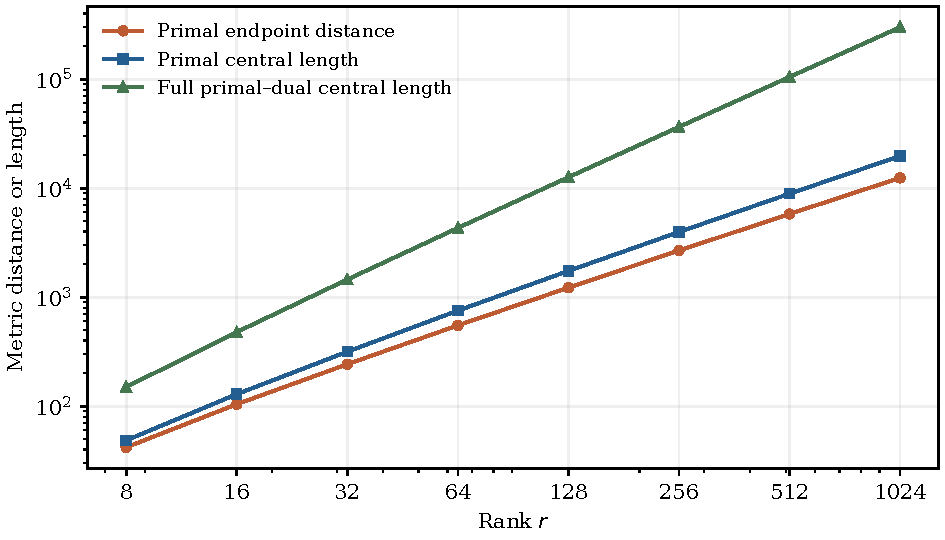
\includegraphics[width=.86\textwidth]{figures/dyadic-lengths.pdf}
 \caption{Numerical values for the dyadic family
 \eqref{eq:dyadic-family}, from $s=0$ to $T=a_r$. The curves show the
 primal endpoint distance $d_U(x^c(0),x^c(T))$ (exact formula), the
 primal central arclength on $[0,T]$ (quadrature), and the full
 central length $\sqrt{2r}\,T$. The first curve is not the distance to
 the whole accurate set, and the third is not the distance to the set
 of feasible small-gap pairs. The orders
 $r\sqrt{\log r}$, $r\log r$, and $r^{3/2}$, and the corresponding step
 counts, follow from \cref{thm:dyadic,thm:completion}.
 Data and generation code accompany the paper.}
 \label{fig:dyadic-lengths}
\end{figure}
